\documentclass{beamer}
\usepackage{hyperref}
\usepackage[T1]{fontenc}
\usepackage{cite}
\usepackage{relsize}
\usepackage{animate}


\usefonttheme[onlymath]{serif}
%C++ symbol
\newcommand{\Rplus}{\protect\hspace{-.1em}\protect\raisebox{.35ex}{\smaller{\smaller\textbf{+}}}}
\newcommand{\Cpp}{\mbox{C\Rplus\Rplus}\hspace{3pt}}
%Scientific notation
\newcommand{\expnumber}[2]{{#1}\mathrm{e}{#2}}

\usepackage{latexsym,amsmath,xcolor,multicol,booktabs,calligra}
\usepackage{graphicx,tikz,listings,stackengine}
\usetikzlibrary{shapes,snakes,matrix, positioning,arrows.meta}
\setbeamertemplate{bibliography item}[text]

\author{Rafael De Luna Loredo}
\title{Programaci\'on en Python y \Cpp}
\subtitle{Estructuras de Datos}
\institute{Facultad de Ciencias, UASLP}
\date{}
\usepackage{NJFU}

% defs
\def\cmd#1{\texttt{\color{red}\footnotesize $\backslash$#1}}
\def\env#1{\texttt{\color{blue}\footnotesize #1}}
\definecolor{deepblue}{rgb}{0,0,0.5}
\definecolor{deepred}{rgb}{0.6,0,0}
\definecolor{deepgreen}{rgb}{0,0.5,0}
\definecolor{halfgray}{gray}{0.55}

\begin{document}
	
	\AtBeginSubsection[]
	{
		\begin{frame}
			\begin{multicols}{3}
				\tableofcontents[currentsection,subsectionstyle=show/shaded/hide,subsubsectionstyle=show/shaded/hide]
			\end{multicols}
		\end{frame}
	}
	\AtBeginSubsubsection[]{
		\begin{frame}
			\begin{multicols}{3}
				\tableofcontents[currentsection,subsectionstyle=show/shaded/hide,subsubsectionstyle=show/shaded/hide]
			\end{multicols}
		\end{frame}
	}
	
	\AtBeginSection[]
	{
		\begin{frame}
			\begin{multicols*}{3}
				\tableofcontents[currentsection,subsectionstyle=show/shaded/hide,subsubsectionstyle=show/shaded/hide]
			\end{multicols*}
		\end{frame}
	}
	
	\begin{frame}
		\titlepage
		\begin{figure}[htpb]
			\begin{center}
				
\includegraphics[width=0.2\linewidth]{fig/logo.png}
			\end{center}
		\end{figure}
	\end{frame}
	
	\begin{frame}{Indice}
		\begin{multicols*}{3}
			\tableofcontents[sectionstyle=show,subsectionstyle=show/shaded/hide,subsubsectionstyle=show/shaded/hide]
		\end{multicols*}
	\end{frame}

\section{Introducci\'on}
\begin{frame}{Introducci\'on}
	\begin{itemize}
		\item Son un grupo o colecci\'on de datos que contienen operaciones para poder manipularlos
		\item Pueden ser est\'aticos o din\'amicos
		\item Nos ayudan a representar datos reales en informaci\'on
		\item Pueden ser lineales o no lineales
	\end{itemize}
\end{frame}

\section{Pilas}
\begin{frame}{Pilas}
	\begin{itemize}
		\item Son una estructura de tipo LIFO (Last In First Out)
		\item Puede ser est\'atica o din\'amica
		\item Cuenta con 2 operaciones b\'asicas
		\item Tiene un tope
		\item Si es est\'atica hay que definir un t\'amaño m\'aximo
	\end{itemize}
\end{frame}

\subsection{M\'etodos}

\begin{frame}{Inserci\'on}
	\begin{itemize}
		\item Hay que comprobar que no este llena
		\item El tope es el nuevo elemento insertado
	\end{itemize}
	\centering
	\animategraphics[autoplay,loop,width=3cm]{20}{animaciones/Estructuras/pilas/insertion/push-}{0}{164}
\end{frame}

\begin{frame}{Eliminaci\'on}
	\begin{itemize}
		\item Hay que comprobar que no este vac\'ia
		\item El nuevo tope ser\'a el elemento debajo del que eliminamos
	\end{itemize}
	\centering
	\animategraphics[autoplay,loop,width=3cm]{20}{animaciones/Estructuras/pilas/elimination/pop-}{0}{164}
\end{frame}

\section{Colas}

\begin{frame}{Colas}
	\begin{itemize}
		\item Son una estructura de tipo FIFO (First In First Out)
		\item Puede ser est\'atica o din\'amica
		\item Cuenta con 2 operaciones b\'asicas
		\item El final es el \'ultimo elemento
		\item Tiene un inicio
		\item Si es est\'atica hay que definir un t\'amaño m\'aximo
	\end{itemize}
\end{frame}

\subsection{M\'etodos}

\begin{frame}{Inserci\'on}
	\begin{itemize}
		\item Hay que comprobar que no este llena
		\item El tope es el nuevo elemento insertado
	\end{itemize}
	\centering
	\animategraphics[autoplay,loop,width=3cm]{20}{animaciones/Estructuras/colas/insertion/qeue-}{0}{164}
\end{frame}

\begin{frame}{Eliminaci\'on}
	\begin{itemize}
		\item Hay que comprobar que no este vac\'ia
		\item El inicio es el elemento siguiente al que eliminamos
	\end{itemize}
	\centering
	\animategraphics[autoplay,loop,width=3cm]{20}{animaciones/Estructuras/colas/elimination/deque-}{0}{149}
\end{frame}

\section{Listas simples}

\begin{frame}{Listas simples}
	\begin{itemize}
		\item Son una estructura lineal
		\item Es din\'amica
		\item Son una colecci\'on de nodos
		\item Cada nodo es un puntero
		\item Cada nodo apunta al que le sigue
	\end{itemize}
	\centering
	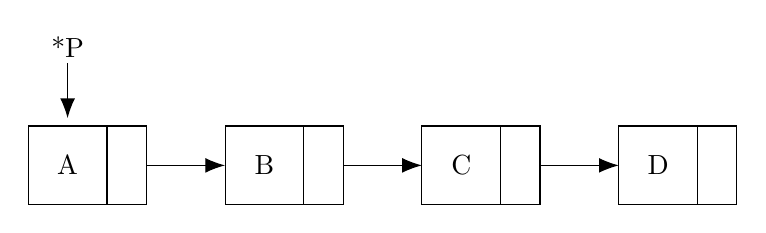
\begin{tikzpicture}
		\node(p) at (0,2) {*P};
		\draw [-{Latex[length=2.5mm]}] (0,1.8) -- (0,1.1);
		\draw (-0.5,0) rectangle +(1,1) (0.5,0) rectangle +(0.5,1);
		\node(p) at (0,0.5) {A};
		\draw [-{Latex[length=2.5mm]}] (1,0.5) -- (2,0.5);
		\draw (2,0) rectangle +(1,1) (3,0) rectangle +(0.5,1);
		\node(p) at (2.5,0.5) {B};
		\draw [-{Latex[length=2.5mm]}] (3.5,0.5) -- (4.5,0.5);
		\draw (4.5,0) rectangle +(1,1) (5.5,0) rectangle +(0.5,1);
		\node(p) at (5,0.5) {C};
		\draw [-{Latex[length=2.5mm]}] (6,0.5) -- (7,0.5);
		\draw (7,0) rectangle +(1,1) (8,0) rectangle +(0.5,1);
		\node(p) at (7.5,0.5) {D};
	\end{tikzpicture}
\end{frame}

\subsection{M\'etodos}

\begin{frame}{Inserci\'on al inicio}
	\begin{itemize}
		\item Si est\'a vac\'ia el nodo ser\'a nulo
		\item Hay que localizar el primer nodo
		\item Creamos un nuevo nodo y apuntara al primer nodo
		\item El nuevo nodo será el primer nodo
	\end{itemize}
	\centering
	\animategraphics[autoplay,loop,width=4cm]{15}{animaciones/Estructuras/listas/simples/insertion/atbegin/begin-}{0}{89}
\end{frame}

\begin{frame}{Inserci\'on al final}
	\begin{itemize}
		\item Hay que localizar el \'ultimo  nodo
		\item Creamos un nodo y el \'ultimo nodo apuntara a este nuevo nodo
		\item El nuevo nodo apuntara a un valor nulo
	\end{itemize}
	\centering
	\animategraphics[autoplay,loop,width=4cm]{15}{animaciones/Estructuras/listas/simples/insertion/end/end-}{0}{89}
\end{frame}

\begin{frame}{Inserci\'on entre nodos}
	\begin{itemize}
		\item Hay que localizar los nodos entre los cu\'ales queremos hacer la inserci\'on
		\item El nodo anterior apunta al nuevo nodo
		\item El nuevo nodo apunta al nodo siguiente
	\end{itemize}
	\centering
	\animategraphics[autoplay,loop,width=4cm]{20}{animaciones/Estructuras/listas/simples/insertion/between/between-}{0}{119}
\end{frame}

\begin{frame}{Eliminaci\'on al inicio}
	\begin{itemize}
		\item Hacemos que el inicio de la lista apunte al siguiente elemento
		\item El inicio ser\'a el elemento siguiente al que eliminamos
		\item Si la lista queda vacía el nodo será nulo
	\end{itemize}
	\centering
	\animategraphics[autoplay,loop,width=4cm]{15}{animaciones/Estructuras/listas/simples/elimination/begin/begin-}{0}{104}
\end{frame}

\begin{frame}{Eliminaci\'on al final}
	\begin{itemize}
		\item Localizamos el \'ultimo
		\item Hacemos que el nodo anterior al \'ultimo sea nulo
		\item Eliminamos el \'ultimo nodo
	\end{itemize}
	\centering
	\animategraphics[autoplay,loop,width=4cm]{15}{animaciones/Estructuras/listas/simples/elimination/end/end-}{0}{119}
\end{frame}

\begin{frame}{Eliminaci\'on entre nodos}
	\begin{itemize}
		\item Localizamos el nodo a eliminar
		\item Hacemos que el nodo anterior apunte al nodo siguiente del que queremos eliminar
		\item Eliminamos el nodo
	\end{itemize}
	\centering
	\animategraphics[autoplay,loop,width=4cm]{10}{animaciones/Estructuras/listas/simples/elimination/between/between-}{0}{44}
\end{frame}

\section{Listas dobles}

\begin{frame}{Listas dobles}
	\begin{itemize}
		\item Tienen dos nodos
		\item Un nodo apunta al siguiente nodo
		\item EL otro nodo apunta al nodo anterior
	\end{itemize}
	\centering
	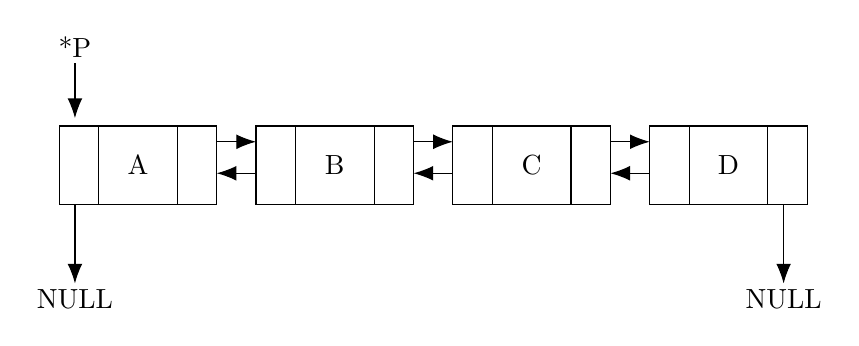
\begin{tikzpicture}
		\node(p) at (-0.8,2) {*P};
		\draw [-{Latex[length=2.5mm]}] (-0.8,1.8) -- (-0.8,1.1);
		\draw (-1,0) rectangle +(0.5,1) (-0.5,0) rectangle +(1,1) (0.5,0) rectangle +(0.5,1);
		\node(null) at (-0.8,-1.2) {NULL};
		\draw [-{Latex[length=2.5mm]}] (-0.8,0) -- (-0.8,-1);
		\node(p) at (0,0.5) {A};
		
		\draw [-{Latex[length=2.5mm]}] (1,0.8) -- (1.5,0.8);
		\draw (1.5,0) rectangle +(0.5,1) (2,0) rectangle +(1,1) (3,0) rectangle +(0.5,1);
		\draw [-{Latex[length=2.5mm]}] (1.5,0.4) -- (1,0.4);
		\node(p) at (2.5,0.5) {B};
		
		\draw [-{Latex[length=2.5mm]}] (3.5,0.8) -- (4,0.8);
		\draw (4,0) rectangle +(0.5,1) (4.5,0) rectangle +(1,1) (5.5,0) rectangle +(0.5,1);
		\draw [-{Latex[length=2.5mm]}] (4,0.4) -- (3.5,0.4);
		\node(p) at (5,0.5) {C};
		
		\draw [-{Latex[length=2.5mm]}] (6,0.8) -- (6.5,0.8);
		\draw (6.5,0) rectangle +(0.5,1)(7,0) rectangle +(1,1) (8,0) rectangle +(0.5,1);
		\draw [-{Latex[length=2.5mm]}] (6.5,0.4) -- (6,0.4);
		\node(p) at (7.5,0.5) {D};
		\node(null) at (8.2,-1.2) {NULL};
		\draw [-{Latex[length=2.5mm]}] (8.2,0) -- (8.2,-1);
	\end{tikzpicture}
\end{frame}

\subsection{M\'etodos}

\begin{frame}{Inserci\'on al inicio}
	\begin{itemize}
		\item Si esta vac\'ia, ambos nodos serán anulos
		\item Localizamos ini \footnote{elemento inicial}
		\item El nodo anterior de ini apuntara al nodo siguiente de ins\footnote{elemento a insertar}
		\item El nodo siguiente de ins apuntara al nodo anterior de ini
		\item El nodo anterior de ins ser\'a nulo
	\end{itemize}
\end{frame}

\begin{frame}{Inserci\'on al final}
	\begin{itemize}
		\item Localizamos fin \footnote{elemento final}
		\item El nodo siguiente de fin apuntara al nodo anterior de ins\footnote{elemento a insertar}
		\item El nodo anterior de ins apuntara al nodo siguiente de fin
		\item EL nodo siguiente de ins ser\'a nulo
	\end{itemize}
\end{frame}

\begin{frame}{Inserci\'on entre nodos}
	\begin{itemize}
		\item Hay que localizar los nodos entre los cu\'ales queremos hacer la inserci\'on \footnote{izq y der}
		\item El nodo siguiente de izq apuntara a nodo anterior de ins \footnote{elemento a insertar}
		\item El nodo anterior de ins apuntara a nodo siguiente de izq
		\item Nodo siguiente de ins apuntara a nodo anterior de der
		\item Nodo anterior de der apuntara a nodo siguiente de ins
	\end{itemize}
\end{frame}

\begin{frame}{Eliminaci\'on al inicio}
	\begin{itemize}
		\item Si quedar\'a vac\'ia la lista apuntar\'a a nulo
		\item Nodo anterior de nwini\footnote{segundo elemento} ser\'a nulo 
		\item Eliminamos nodo siguiente de elim\footnote{elemento a eliminar}
	\end{itemize}
\end{frame}

\begin{frame}{Eliminaci\'on al final}
	\begin{itemize}
		\item Localizamos fin
		\item Hacemos nodo siguiente de nwfin\footnote{elemento anterior a fin} nulo
		\item Hacemos nulo al nodo anterior de fin
	\end{itemize}
\end{frame}

\begin{frame}{Eliminaci\'on entre nodos}
	\begin{itemize}
		\item Localizamos elim
		\item Nodo siguiente de der apunta a nodo anterior de izq
		\item Nodo anterior de izq apunte a izq\nocite{BHASIN,BJARNE1,BJARNE2,CAIRO,CPP,DEITEL,DOWNEY,JAWORSKI,KENN,lAAKMANN,MATTHES,RAMALHO,SED,BRASSARD,CAIRO2}
	\end{itemize}
\end{frame}

\section{Arboles}

\begin{frame}{Arboles}
	Son estructuras din\'amicas no lineales ordenadas y una de las mas importantes en computaci\'on.
	Pueden cambiar tanto de forma como de tamaño durante la ejecuci\'on.\\
	\centering
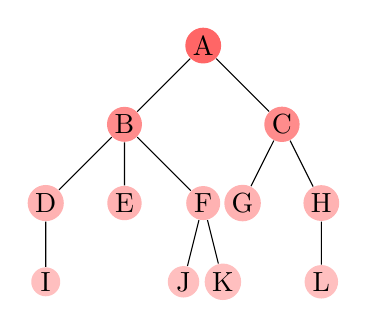
\begin{tikzpicture}
	[level distance=10mm,
	every node/.style={fill=red!60,circle,inner sep=1pt},
	level 1/.style={sibling distance=20mm,nodes={fill=red!45}},
	level 2/.style={sibling distance=10mm,nodes={fill=red!30}},
	level 3/.style={sibling distance=5mm,nodes={fill=red!25}}]
	\node {A}
	child {node {B} 
		child {node {D}
			child {node {I}}
		}
		child {node {E}
			child[missing]
		}
		child {node {F}
			child {node {J}}
			child {node {K}}
		}
	}
	child {node {C}
		child {node {G}
			child[missing]
		}
		child {node {H}
			child {node {L}}
		}
	};
\end{tikzpicture}
\end{frame}

\begin{frame}[allowframebreaks]
	\frametitle{Conceptos clave}
	\begin{itemize}
		\item \textbf{Ra\'iz}: Es el nodo principal o inicial
		\item \textbf{Padre}:  Un nodo que apunta hacia otros nodos
		\item \textbf{Hijo}:  Un nodo que es apuntado por otro nodo
		\item \textbf{Hoja}:  Nodo sin hijos
		\item \textbf{Nodo interior}: Nodo que no es ra\'iz ni hoja
		\item \textbf{Grado}: Numero de hijos de un nodo
		\item \textbf{Grado del \'arbol}: M\'aximo grado de todos los nodos del \'arbol
		\item \textbf{Brazo}: Conexi\'on entre un nodo y otro
		\item \textbf{Camino}: Secuencia de nodos y brazos conectados por un hijo
		\item \textbf{Nivel}:  N\'umero de brazos entre un nodo y la ra\'iz mas uno
		\item \textbf{Altura}: N\'umero de brazos entre en el camino mas largo entre un nodo y una hoja.
		\item \textbf{Altura del \'arbol}:  Altura del nodo ra\'iz
		\item \textbf{Profundidad}: N\'umero de brazos desde la ra\'iz hasta un nodo
		\item \textbf{Rama}: Una ruta de la ra\'iz a cualquier nodo  
	\end{itemize}
\end{frame}

\subsection{Arboles binarios (ABB)}

\begin{frame}{Arboles binarios}
	Son \'arboles de grado 2 donde cada nodo  tiene m\'aximo dos sub\'arboles, siendo sub\'arbol izquierdo y derecho respectivamente., a la derecha se van colocando los valores mayores que la ra\'iz y a la izquierda los menores.
\end{frame}

\subsubsection{Operaciones}

\begin{frame}{Inserci\'on}
	\begin{itemize}
		\item Si est\'a vac\'io la ra\'iz apunta a null
		\item Si insertamos un elemento en un \'arbol vac\'io, ra\'iz apuntara a este nuevo elemento y sus dos sub\'arboles apuntaran a null
		\item  Si no est\'a vac\'io comparamos el nuevo valor a insertar con la ra\'iz, y vamos comparando con cada nodo seg\'un corresponda
	\end{itemize}
\end{frame}

\begin{frame}{Recorrido en preorden}
	\begin{itemize}
		\item Visitamos la ra\'iz
		\item Recorremos el sub\'arbol izquierdo
		\item Recorremos el sub\'arbol derecho
	\end{itemize}
\end{frame}

\begin{frame}{Recorrido en inorden}
	\begin{itemize}
		\item Recorremos el sub\'arbol izquierdo
		\item Visitamos la ra\'iz
		\item Recorremos el sub\'arbol derecho
	\end{itemize}
\end{frame}

\begin{frame}{Recorrido en posorden}
	\begin{itemize}
		\item Recorremos el sub\'arbol izquierdo
		\item Recorremos el sub\'arbol derecho
		\item Visitamos la ra\'iz
	\end{itemize}
\end{frame}


\subsection{Arboles AVL}

\begin{frame}{Arboles balanceados}
	Son \'arboles que despu\'es de una inserci\'on o eliminaci\'on se reacomodan manteniendo una diferencia de altura menor o igual 1 entre las ramas derecha e izquierda.
\end{frame}

\begin{frame}{Ventajas respecto a \'arboles binarios}
	Los \'arboles balanceados surgieron como una soluci\'on a un problema que tienen los ABB, y es que si en un ABB se insertan datos ordenados de manera ascendente o descendente, estos crecer\'an de manera descontrolada.
\end{frame}

\subsection{Arboles B}
\begin{frame}{Arboles B}
	Son una generalizaci\'on de los \'arboles AVL y representan un m\'etodo para almacenar y recuperar informaci\'on en medios externos.
\end{frame}

\begin{frame}{Caracter\'isticas}
	\begin{itemize}
		\item Un grupo de nodos se llama p\'agina
		\item En cada p\'agina se almacena la informaci\'on del grupo de nodos y se identifica por medio de claves o llaves.
		\item Cada p\'agina, excepto la ra\'iz contiene \textbf{d} y \textbf{2d} elementos, siendo \textbf{d} el grado del \'arbol
		\item La p\'agina ra\'iz tiene al menos dos descendientes
		\item Las p\'aginas hoja est\'an todas al mismo nivel
		\item Crecen de las hojas hacia la ra\'iz
	\end{itemize}
\end{frame}

\subsection{Arboles B+}

\begin{frame}{Arboles B+}
	Son muy parecidos a los \'arboles b con la diferencia de que la informaci\'on se encuentra en las hojas, mientras que los nodos ra\'iz e interiores almacenan claves que se utilizan como \'indices.
\end{frame}

\begin{frame}{Ventajas respecto a \'arboles B}
	Pese a que ocupan un poco mas de espacio debido a la duplicidad en algunas claves, esto es aceptable si el archivo se modifica frecuentemente, ya que esto evita la reorganizaci\'on.
\end{frame}

\begin{frame}{Caracter\'isticas}
	\begin{itemize}
		\item Cada p\'agina, excepto la ra\'iz contiene \textbf{m} elementos, donde  \textbf{m} es un elemento entre \textbf{d} y \textbf{2d}
		\item La ra\'iz tiene entre 1 a \textbf{2d}
		\item Cada p\'agina, excepto la ra\'iz, tiene entre \textbf{d} $+ 1$ y \textbf{2d} $+ 1$ descendientes
		\item La ra\'iz tiene al menos dos descendientes
		\item Las hojas est\'an todas al mismo nivel
		\item Toda la informaci\'on, con las claves que las identifican, se encuentran en las hojas
		\item Las claves en la ra\'iz y p\'aginas interiores se utilizan como \'indices
	\end{itemize}
\end{frame}

\section{Referencias}
\subsection{}
\begin{frame}[allowframebreaks]
	\frametitle{Referencias}
	\bibliographystyle{acm}
	\bibliography{ref.bib}
\end{frame}

\end{document}
